\documentclass[11pt, a4paper]{article}

\usepackage[T1]{fontenc}
\usepackage[utf8]{inputenc}
\usepackage[polish]{babel}
\usepackage{listings}
\usepackage{mathtools}
\usepackage{blindtext}
\usepackage{scrextend}
\usepackage{graphicx}
\usepackage{hyperref}


\graphicspath{ {./images/} }


\begin{document}

\title{Niskopoziomowa implementacja konwolucyjnej sieci neuronowej}
\author{Kacper Janda}
\date{}
\maketitle

\section{Założenia projektu}
\begin{center}
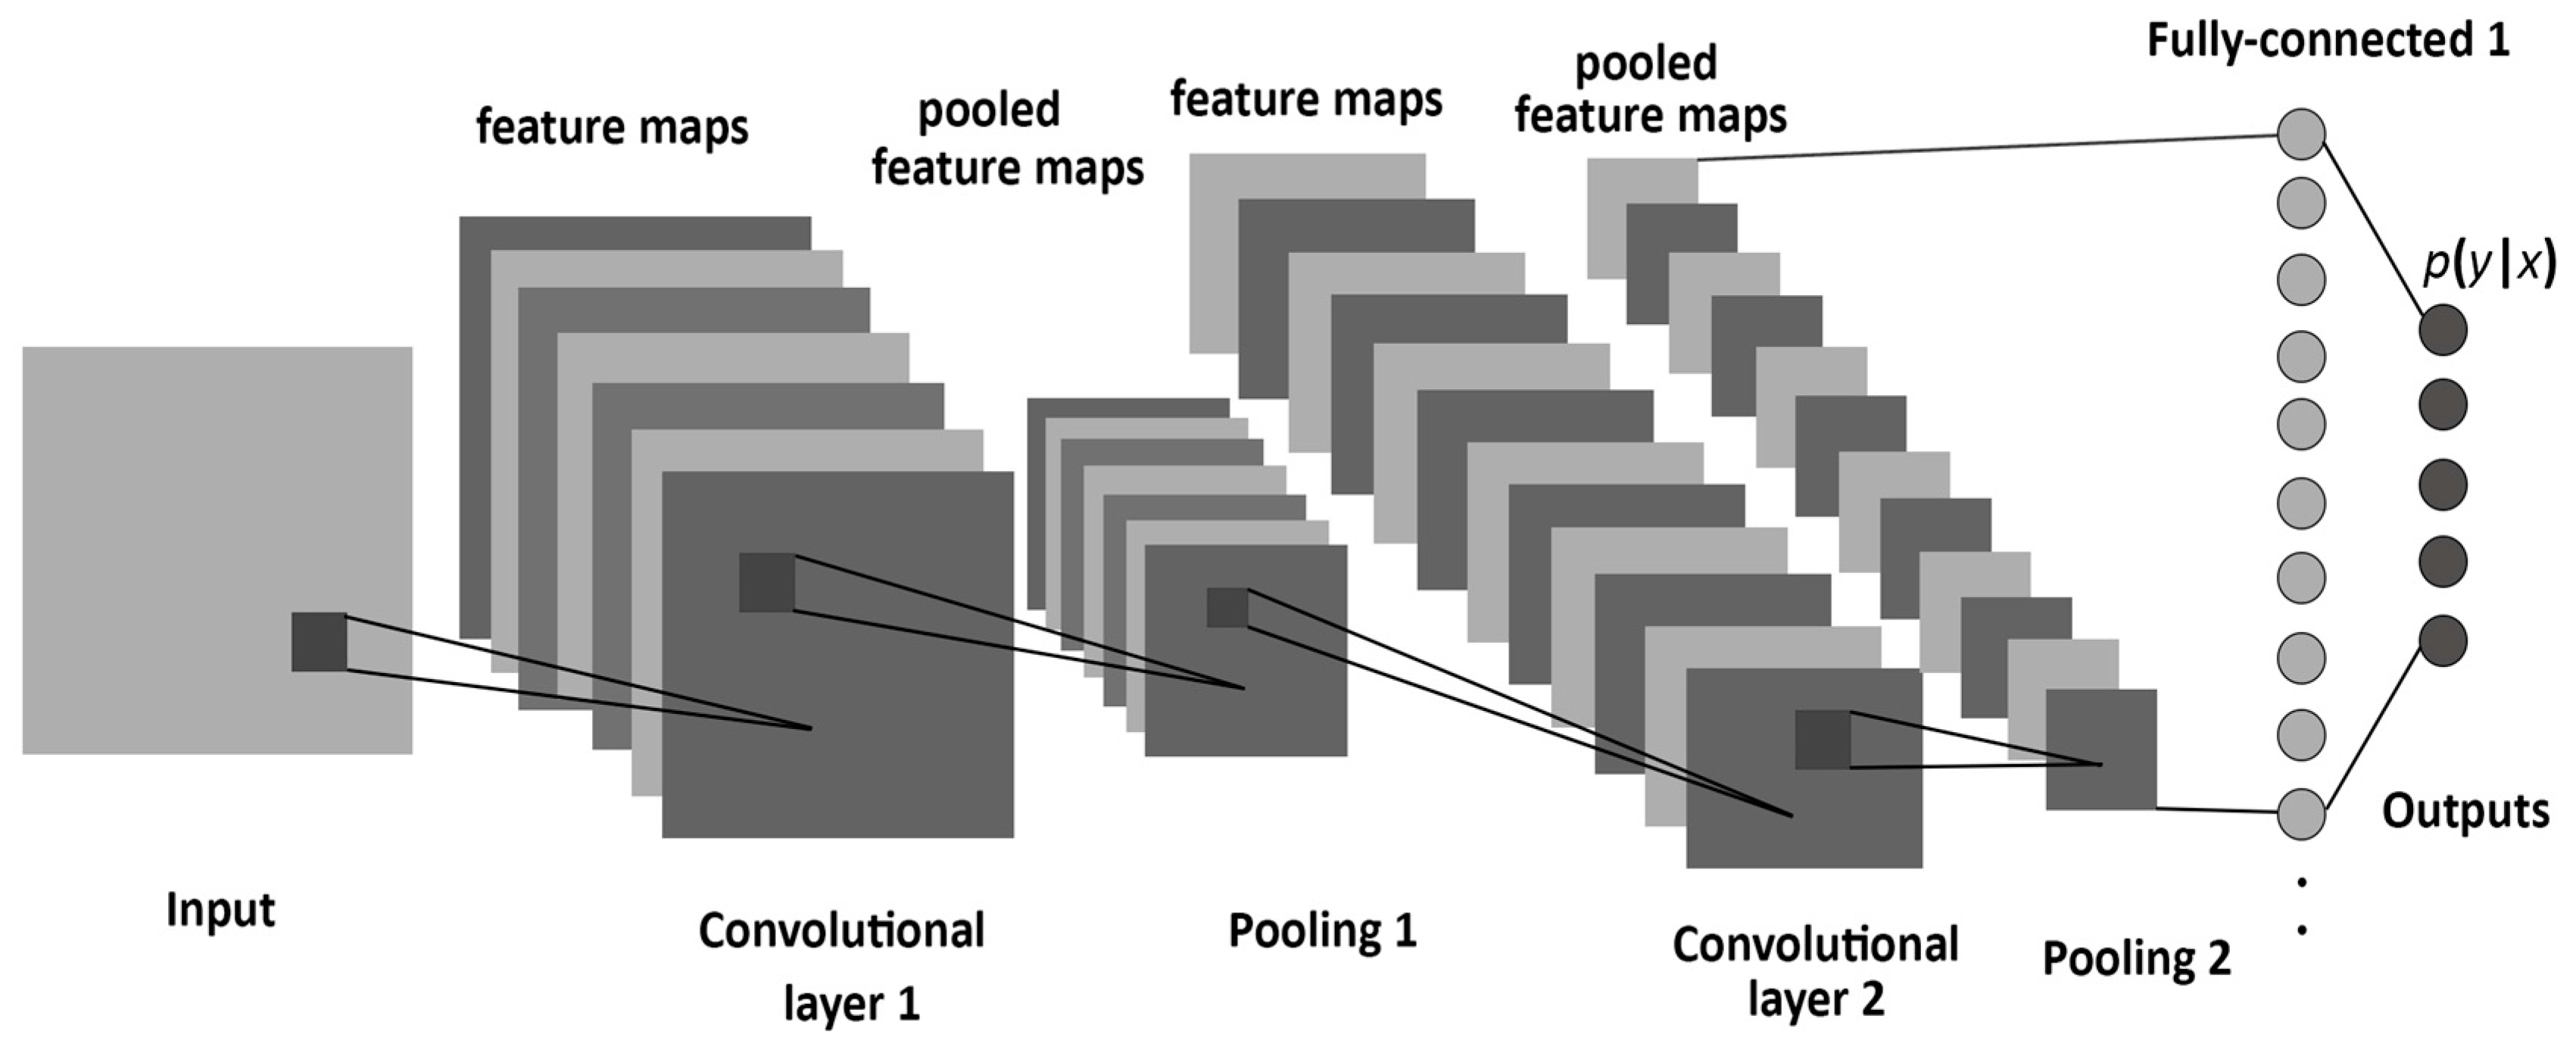
\includegraphics[scale=0.6]{CNN.png}
\end{center}\
Celem projektu jest stworzenie działającej konwolucyjnej sieci neuronowej, która będzie służyła do rozpoznawania cyfr na podstawie zdjęć. Poza obsługą kamery oraz konwersją zdjęcia na bitmapę projekt zostanie wykonany w całości niskopoziomowo.
\section{Plan prac}
\begin{enumerate}
\item Zdobycie niezbędnej wiedzy w zakresie konwolucyjnych sieci neuronowych
\item Projekt struktury sieci
\item Implementacja niezbędnych funkcji matematycznych oraz obsługa parsowania danych testowych
\item Implementacja mechanizmów konwolucyjnej sieci neuronowej
\item Implementacja konwersji zdjęć do odpowiedniej postaci
\item Testy oraz optymalizacja działania
\end{enumerate}
\section{Wykorzystane narzędzia}
\begin{enumerate}
\item Język C
\item Baza danych testowych MNIST
\end{enumerate}
\section{Postęp prac}
\begin{enumerate}

\item W pierwszym tygodniu udało mi się zaimplementować bibliotekę do operacji na macierzach, pozostałe funkcje matematyczne oraz niektóre funkcje do obsługi sieci.

\item Następnie rozpocząłem pracę nad funkcjami związanymi z uczeniem sieci. Wymagało to dużej ilości czasu w związku z potrzebą zaznajomienia się z tematem. W trzecim tygodniu prac udało mi się skończyć implementację logiki sieci. Korzystając z narzędzia Sanitizer naprawiłem wszystkie wycieki pamięci. Pierwsze testy wypadły dość optymistycznie.  

\end{enumerate}

\section{Bibliografia}
\url{http://neuralnetworksanddeeplearning.com/chap1.html}\\\\
\url{https://grzegorzgwardys.wordpress.com/2016/04/22/8}\\\\
\url{https://medium.com/the-bioinformatics-press/only-numpy-understanding-back-propagation-for-max-pooling-layer-in-multi-layer-cnn-with-example-f7be891ee4b4}\\\\
\url{https://www.jefkine.com/general/2016/09/05/backpropagation-in-convolutional-neural-networks/}\\\\
\url{https://www.youtube.com/watch?v=EjzrnqlWYYY&t=695s}

\end{document}